\documentclass{standalone}
\usepackage{pgfplots}
\pgfplotsset{compat=newest}

\begin{document}
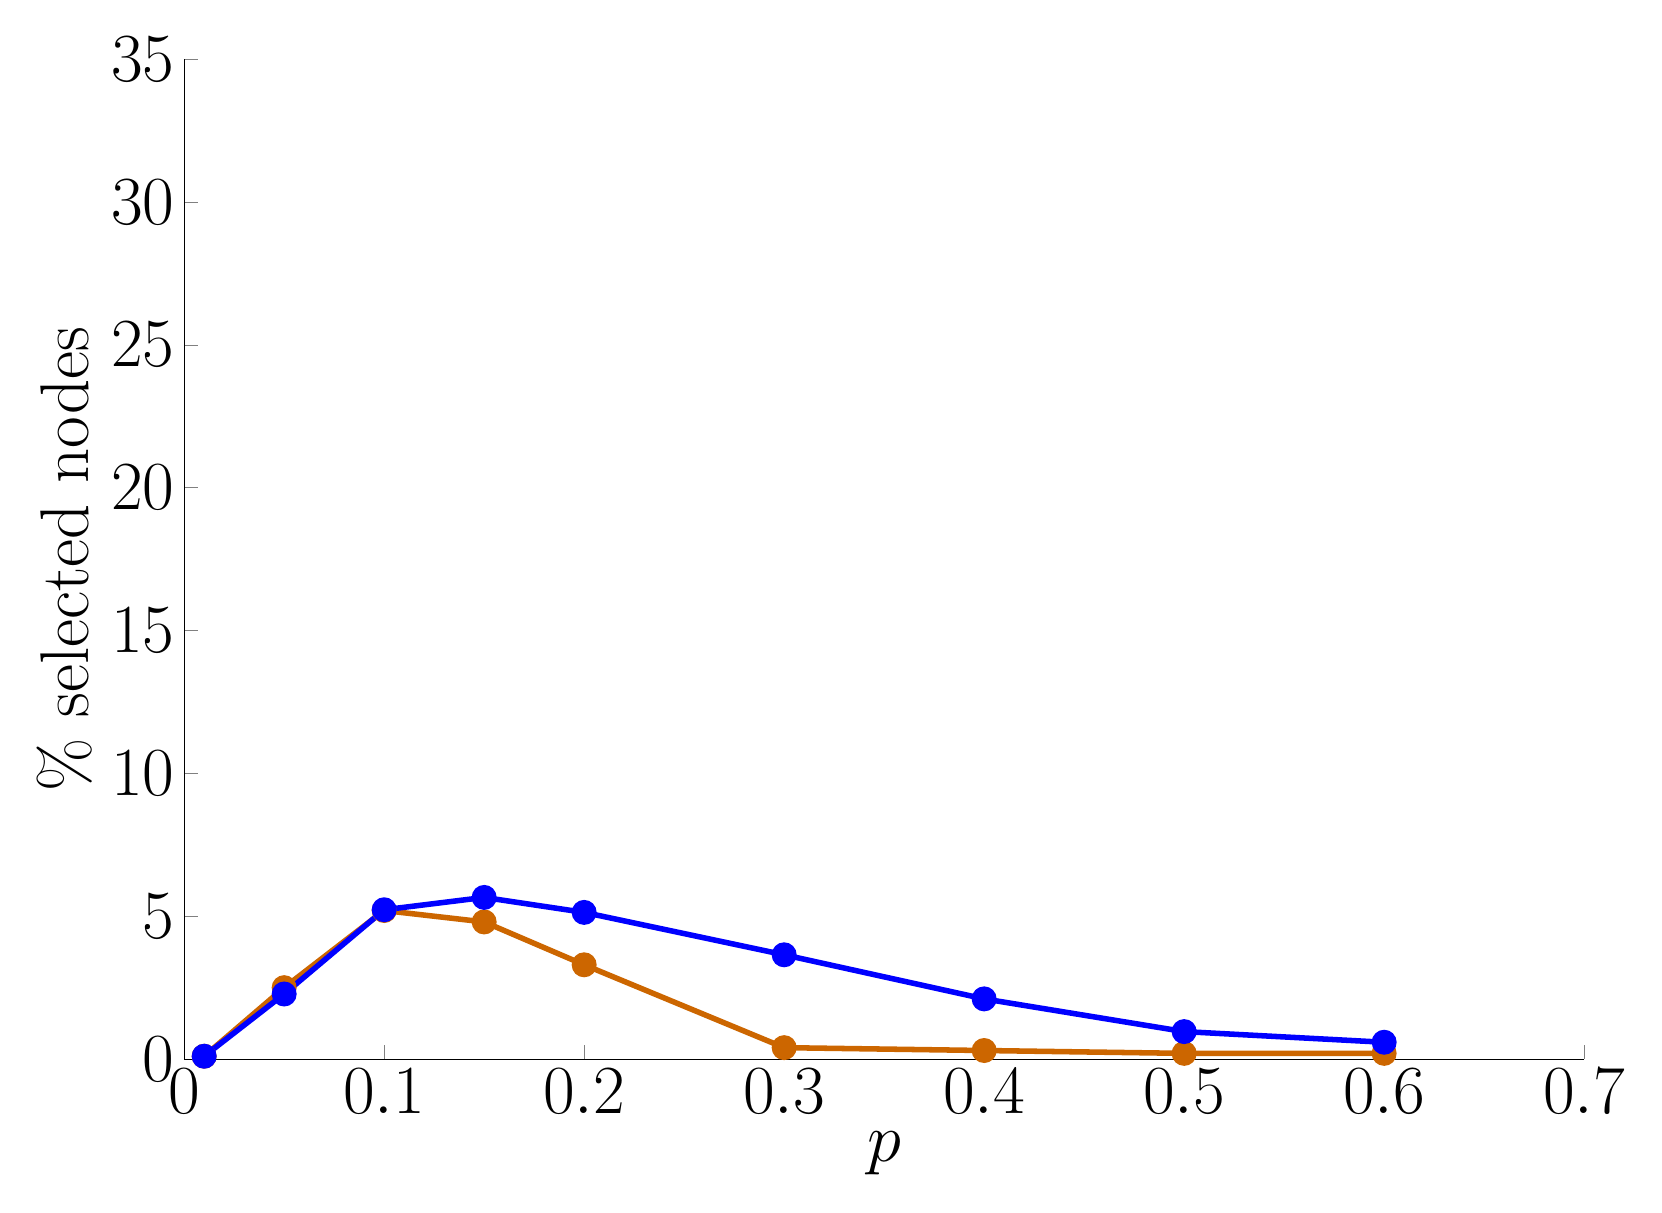
\begin{tikzpicture}

\begin{axis}[%
tick label style={font=\Huge},
label style={font=\Huge},
legend style={font=\Huge},
view={0}{90},
width=7in,
height=5in,
scale only axis,
xmin=0, xmax=0.7,
xtick={0, 0.1, 0.2, 0.3, 0.4, 0.5, 0.6, 0.7},
xlabel={$p$},
ymin=0, ymax=35,
ytick={0, 5, 10, 15, 20, 25, 30, 35},
ylabel={$\%$ selected nodes},
major tick length=5pt,
axis lines*=left,
legend cell align=left,
clip=false]

\addplot [
mark=*,
mark size=3.5pt,
color=orange!80!black,
solid,
line width=2pt,
]
coordinates{
(0.01,0.1)(0.05,2.5)(0.1,5.2)(0.15,4.8)(0.2,3.3)(0.3,0.4)(0.4,0.3)(0.5,0.2)(0.6,0.2)
};

\addplot [
mark=*,
mark size=3.5pt,
color=blue,
solid,
line width=2pt,
]
coordinates{
(0.01,0.1)(0.05,2.278)(0.1,5.226)(0.15,5.658)(0.2,5.134)(0.3,3.65)(0.4,2.107)(0.5,0.962)(0.6,0.589)
};

\end{axis}
\end{tikzpicture}
\end{document}
